\begin{frame}{Coding Theory}
    \begin{itemize}
        \item The study of the properties of codes and their respective fitness for specific applications.
    \end{itemize}
    \begin{columns}
        \begin{column}{0.5\textwidth}
            \begin{figure}
            \centering
                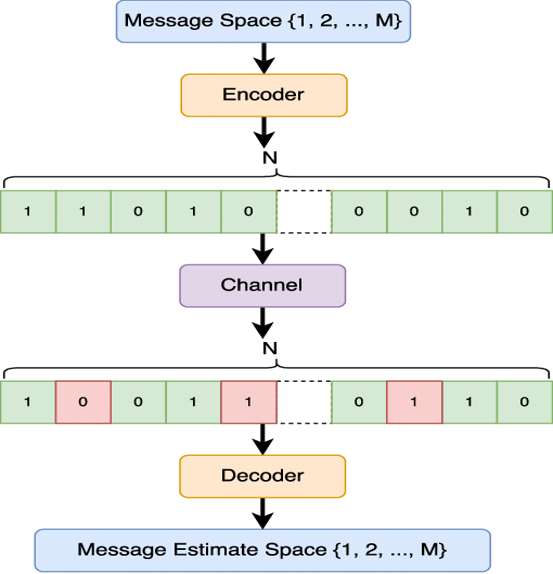
\includegraphics[width=0.8\textwidth]{Images/Introduction/CodingTheory.png}
                \caption{Coding Process.}
                \label{fig:coding_process}
            \end{figure}
        \end{column}
        
        \begin{column}{0.5\textwidth}
            \begin{figure}
                \centering
                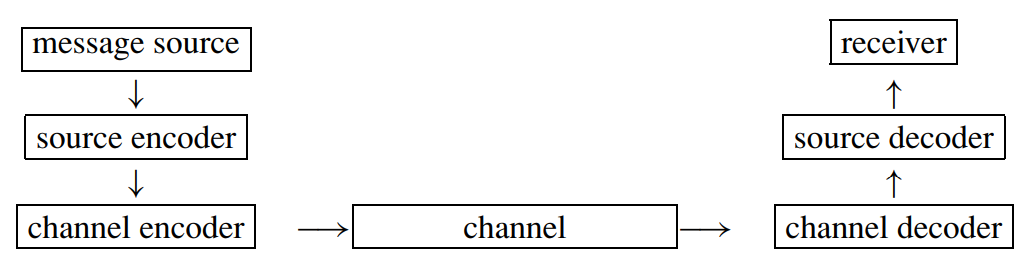
\includegraphics[width=\textwidth]{Images/Introduction/sourceandchannelcoding.png}
                \caption{Source and Channel Coding.}
                \label{fig:sourcechannelcoding}
            \end{figure}    
        \end{column}    
    \end{columns}
\end{frame}

\begin{frame}{Coding Theory - Applications}
    \begin{columns}
        \begin{column}{0.5\textwidth}
            \begin{itemize}
                \vfill \item Run length limited code is used in CD, DVD.
                \begin{figure}
                    \centering
                    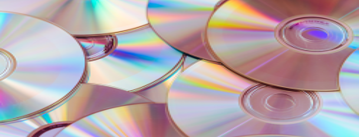
\includegraphics[width=0.7\textwidth]{Images/Introduction/CDDVD.png}
                    % \caption{Caption}
                    % \label{fig:my_label}
                \end{figure}
                \hfill
                \vfill \item 3G,4G networks use Reed- Solomon code.
                \begin{figure}
                    \centering
                    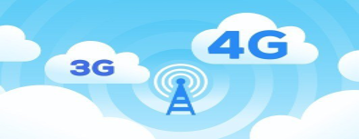
\includegraphics[width=0.7\textwidth]{Images/Introduction/3G4G.png}
                    % \caption{Caption}
                    % \label{fig:my_label}
                \end{figure}
                \vfill \item 5G networks use Turbo code.
                \begin{figure}
                    \centering
                    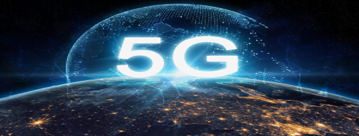
\includegraphics[width=0.7\textwidth]{Images/Introduction/5G.png}
                    % \caption{Caption}
                    % \label{fig:my_label}
                \end{figure}
            \end{itemize}
        \end{column}
        
        \begin{column}{0.5\textwidth}
            \begin{itemize}
                \vfill \item LDPC code is used in Data modems, telephone transmissions, and the NASA Deep Space Network.
                \begin{figure}
                    \centering
                    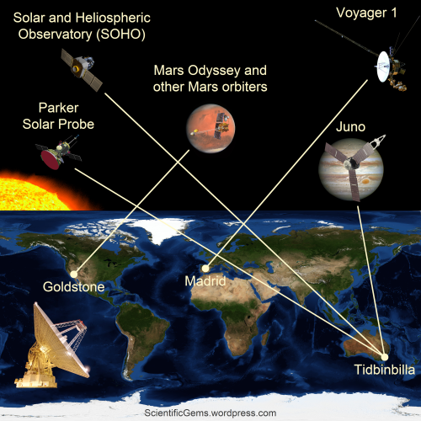
\includegraphics[width=0.8\textwidth,height=0.6\textheight]{Images/Introduction/NASA.png}
                    % \caption{Caption}
                    % \label{fig:my_label}
                \end{figure}
            \end{itemize}
        \end{column}
    \end{columns}
\end{frame}


\begin{frame}{Constrained Code}
    \begin{itemize}
        \vfill \item Code: set of (binary) sequences, strings.
        
        $\rightarrow$ Constrained code $\mathbb{C}$: set of sequences satisfying given constraints.
        \vfill \item Presentation: a directed graph $G=(V,E)$.
        \vfill \item Path: sequence of edges $\left(e_{1},e_{2},\ldots,e_{n}\right)$ such that the end vertex of $e_{i}$ is the start vertex of $e_{i+1}$ $e_{i}\in E$. 
        \vfill \item Simple path: path with no repeated edges.
    \end{itemize}
\end{frame}

\begin{frame}{De Bruijn Code (Positioning Code)}
    \begin{columns}
        \begin{column}{0.65\textwidth}
            \begin{enumerate}
                \item De Bruijn graph of order $k$, $G_{k}$:
                \begin{itemize}
                    \item Each vertex is labeled by a sequence of length $k-1$.
                    \item A directed edge from $\bfx = \left[x_{0}x_{1}\ldots x_{k-2}\right]$ to $\bfy=\left[y_{0}y_{1}\ldots y_{k-2}\right]$ $\Leftrightarrow\ x_{1}x_{2}\ldots x_{k-2}=y_{0}y_{1}\ldots y_{k-3}$. 
                \end{itemize}
                \item De Bruijn sequence:
                \begin{itemize}
                    \item A cyclic binary de Bruijn of order $k$ is a length $2^{k}$ sequence such that each length $k$ string appears exactly once.
                    \item Longest simple path in de Bruijn graph (Eulerian cycle) $\equiv$ de Bruijn sequence.
                \end{itemize}
                
                \item Applications:
                \begin{itemize}
                    \item Cryptography.
                    \item Interconnection networks.
                    \item VLSI testing.
                    \item Combine with biology: DNA storage.
                \end{itemize}
            \end{enumerate}
        \end{column}
        
        \begin{column}{0.35\textwidth}
            \begin{figure}
                \centering
                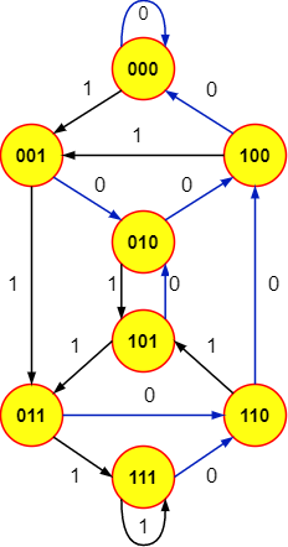
\includegraphics[width=0.8\textwidth]{Images/deBruijnOrder4.png}
                \caption{de Bruijn graph of order $4$.}
                \label{fig:dB4}
            \end{figure}
        \end{column}
    \end{columns}
\end{frame}

\begin{frame}{What do we concern about a code?}
    \begin{block}<1>{Rate}
        Rate and Maximal asymptotic rate tend to as high as possible.
    \end{block}
    \begin{block}<1>{Efficient encoding algorithm}
        Encoding algorithm: maps messages into codewords, generates sequences in the code, \dots.
    \end{block}
    \begin{block}<1>{Efficient decoding algorithm}
        Decoding algorithm: maps codewords into messages, locates the position of the sequences in the ordered code, \dots.
    \end{block}
    \begin{block}<0>{Et Cetera}
        Fault tolerant, robust positioning, \dots.
    \end{block}
\end{frame}